\newpage % Эта команда начинает новую страницу
\chapter{Виртуальная машина Java}% Эта команда начинает первую лекцию. В фигурных скобках нужно
% записать тему лекции. Эта тема лекции автоматически получит порядковый номер и
% автоматически добавится в раздел <<Содержание>>. Лекций можно создавать сколько угодно.
% Для создания новой лекции скопируйте и вставьте (или наберите с клавиатуры) команду
% \chapter{Тема лекции} в любую часть рабочего файла. Можете смело менять местами лекции --
% вся нумерация после очередной компиляции поменяется автоматически.

% При необходимости здесь можно разместить любой текст

\section{Виртуальные машины Java и .NET}% Эта команда начнет раздел, который будем далее условно называть
% параграф. В роли параграфа будет выступать структурная часть лекции (отдельный раздел,
% вопрос и т.п.). В фигурных скобках нужно вписать название параграфа. Параграф автоматически
% получит порядковый номер, который будет состоять из двух чисел, разделенных точкой.
% Первое число -- порядковый номер лекции, второе число -- порядковый номер параграфа в
% пределах лекции. Параграфов можно создавать сколько угодно. Для создания нового параграфа
% скопируйте и вставьте (или наберите с клавиатуры) команду \section{Название параграфа} в
% любую часть рабочего файла. Можете смело менять местами параграфы, переносить их из одной
% лекции  в другую -- вся нумерация после очередной компиляции поменяется автоматически.

% При необходимости здесь можно разместить любой текст

% Эта команда начинает подраздел, который далее будем
% условно называть подпараграфом. В фигурных скобках нужно вписать название подпараграфа.
% Подпараграф автоматически получит порядковый номер, который будет состоять из трех
% чисел, разделенных точками. Первое число -- порядковый номер лекции, второе число --
% порядковый номер параграфа, третье число -- порядковый номер подпараграфа. Подпараграфов
% можно создавать сколько угодно. Для создания нового подпараграфа скопируйте и вставьте
% (или наберите с клавиатуры) команду \subsection{Название подпараграфа} в любую часть
% Рабочего файла. Можете смело менять подпараграфы местами, переносить их из одного
% параграфа в другой (даже другой параграф другой лекции) -- вся нумерация после очередной
% компиляции поменяется автоматически.

Виртуальные машины Java и .NET - это программные среды, которые позволяют выполнять приложения, написанные на языках программирования Java и .NET, соответственно, на любой операционной системе, где установлена соответствующая виртуальная машина.

\textbf{Виртуальная машина Java (JVM)} - это программная среда, которая выполняет байт-код, созданный компилятором Java. Байт-код - это промежуточный код, который создается компилятором Java из исходного кода программы на Java. JVM интерпретирует этот байт-код и выполняет его на любой платформе, где установлена JVM. Благодаря JVM, приложения на Java могут быть написаны один раз и выполняться на любой платформе без необходимости переписывания кода.

\textbf{Виртуальная машина .NET (CLR)} - это программная среда, которая выполняет код, написанный на языках программирования, которые поддерживают .NET Framework, таких как C#, F# и Visual Basic. Код на этих языках компилируется в промежуточный язык (IL), который затем выполняется на CLR. CLR предоставляет среду выполнения для .NET Framework, включая управление памятью, обработку исключений и динамическую компиляцию.

Виртуальные машины Java и .NET позволяют разработчикам писать кроссплатформенные приложения, что означает, что один и тот же код может быть запущен на любой операционной системе, где установлена соответствующая виртуальная машина. Кроме того, эти виртуальные машины также предоставляют богатый набор библиотек и классов, которые упрощают разработку приложений.

Однако, использование виртуальных машин также может снизить производительность приложений, поскольку промежуточный код должен быть интерпретирован или скомпилирован в рантайме. Также использование виртуальных машин может требовать дополнительных ресурсов, таких как оперативная память и процессорное время.

\section{Структура виртуальной машины}

Структура виртуальной машины Java (Java Virtual Machine, JVM) включает в себя следующие компоненты:
\begin{enumerate}
\item Класс-лоадеры - компоненты, которые загружают и инициализируют классы в JVM. Класс-лоадеры используют иерархическую систему для загрузки классов, которая обеспечивает безопасность и защиту от конфликтов.
\item Память - виртуальная машина Java использует четыре области памяти: куча (heap), стек (stack), область методов (method area) и область постоянного памяти (permanent generation). Куча используется для хранения объектов, стек используется для хранения вызовов методов, область методов используется для хранения байт-кода, а область постоянного памяти используется для хранения метаданных и других информационных ресурсов.
\item Интерпретатор - компонент, который читает байт-код и выполняет соответствующие операции.
\item Оптимизатор - компонент, который оптимизирует байт-код, чтобы улучшить производительность.
\item Сборщик мусора - компонент, который автоматически освобождает память, занятую объектами, которые больше не используются.
\item Библиотеки и классы - виртуальная машина Java предоставляет библиотеки и классы, которые могут быть использованы программистами для упрощения разработки приложений.
\end{enumerate}

\begin{figure}[h!]\center
  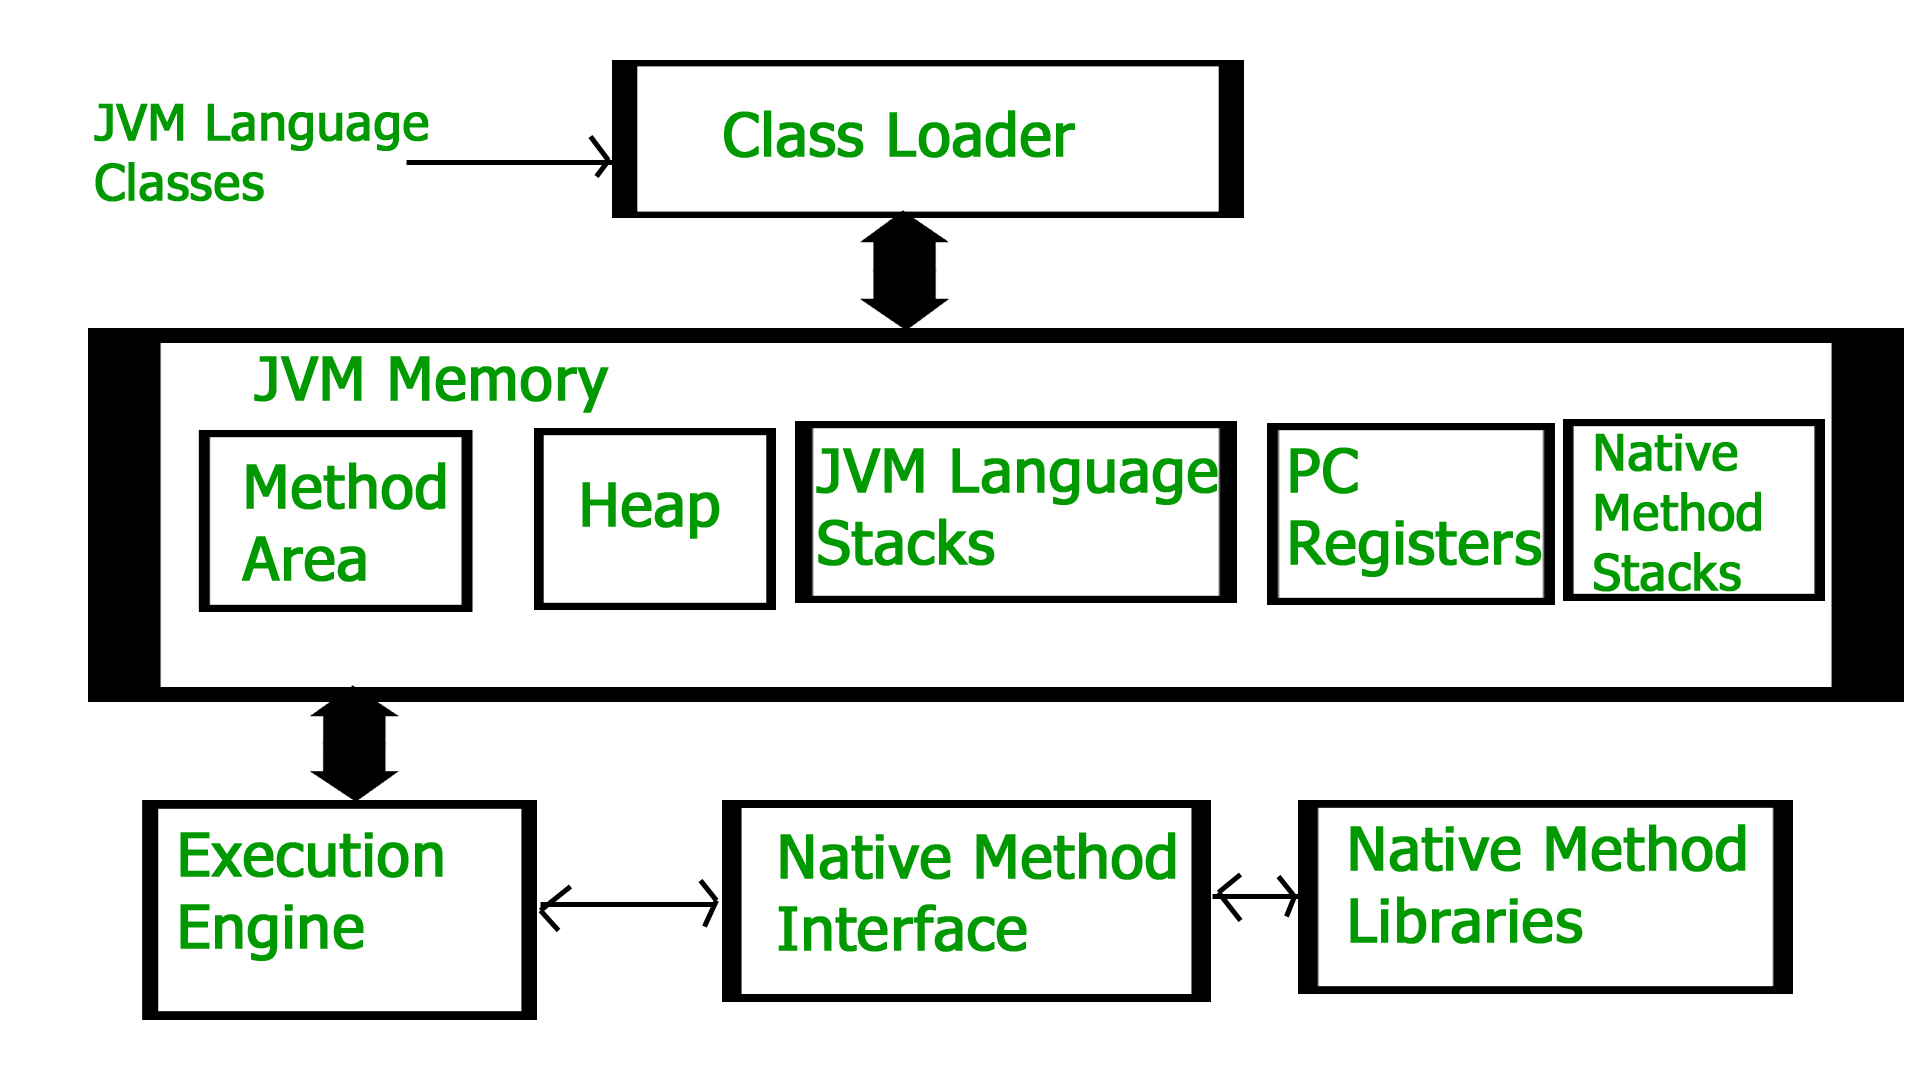
\includegraphics[width=0.8\linewidth]{images/pic1-1.jpg}
   \caption{Структура виртуальной машины Java}\label{ris1}
\end{figure}

Каждый запущенный Java-процесс имеет свою собственную виртуальную машину Java. JVM работает как посредник между Java-программой и операционной системой, обеспечивая переносимость и безопасность Java-программ. Благодаря этому, Java-программы могут выполняться на любой операционной системе, для которой существует виртуальная машина Java.

\section{Этапы сборки программного проекта и роль виртуальной машины}

\textbf{Сборка (англ. assembly)} — двоичный файл, содержащий исполняемый код программы или (реже) другой подготовленный для использования информационный продукт.

\textbf{Автоматизация сборки} — этап написания скриптов или автоматизация широкого спектра задач применительно к ПО, применяемому разработчиками в их повседневной деятельности, включая такие действия, как:
\begin{enumerate}
\item Компиляция исходных файлов: Исходные файлы программы (.java) компилируются в байт-код (.class) с помощью компилятора javac. Компилятор проверяет синтаксис кода, а также проверяет, чтобы все классы и методы были объявлены и использованы правильно.
\item Создание jar-файла: Компилированные .class-файлы собираются в jar-файл, который является архивом, содержащим все необходимые классы, библиотеки и ресурсы.
\item Тестирование: Запуск программы на предмет выявления ошибок и неполадок.
\item Упаковка и развертывание: Упаковка программы в приложение, которое может быть запущено на других машинах. Это может включать в себя создание установочных файлов или деплоя на сервер.
\item Поддержка и обновление: Поддержка и обновление программы после ее выпуска, включая исправление ошибок, улучшение производительности и добавление новых функций.
\end{enumerate}

Для автоматизации сборки проектов традиционно используют системы сборки, такие как make на Unix подобных системах и nmake для компилятора Microsoft. Также традиционно написание файлов для сборки проекта под эти системы является задачей нетривиальной. Конечно, пользуясь только Mictosoft Visual Studio можно даже не подозревать о существовании этих файлов, так как интегрированная среда разработки достаточно удобно скрывает всю схему работы, оставляя снаружи несколько диалоговых окон и кнопку Build. Но для сложных проектов использующих массу сторонних библиотек и кроссплатформенных проектов такой подход часто оказывается неприемлемым.

\textbf{Роль Java Virtual Machine}

\begin{figure}[h!]\center
  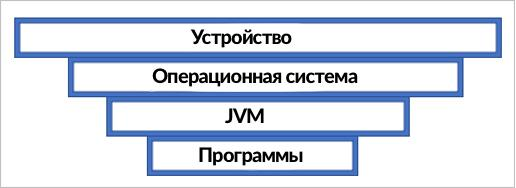
\includegraphics[width=0.8\linewidth]{images/pic1-2.jpg}
\end{figure}

Если вы внимательно посмотрите на схему, добавленную ниже, то будет несложно догадаться, что JVM образует слой между операционной системой и программами Java.

Это означает, что скомпилированная Java-программа будет связываться с Java Virtual Machine, а JVM будет общаться с операционной системой, являясь своего рода посредником между скомпилированными файлами классов и операционной системой.

Виртуальная машина (Virtual Machine, VM) является ключевым компонентом в экосистеме языка Java, и выполняет множество важных функций:
\begin{enumerate}
\item Интерпретация байт-кода: Когда Java-приложение запускается, байт-код (.class-файлы) не выполняется напрямую на операционной системе, а передается на исполнение виртуальной машине. Виртуальная машина интерпретирует байт-код и выполняет соответствующие инструкции на операционной системе.
\item Платформонезависимость: Виртуальная машина Java обеспечивает платформонезависимость Java-приложений. Так как байт-код может быть запущен на любой платформе, которая поддерживает Java-виртуальную машину, разработчики могут создавать приложения, которые могут работать на разных операционных системах, не переписывая их для каждой платформы.
\item Менеджмент памяти: Виртуальная машина управляет памятью, выделяя и освобождая память для объектов, создаваемых приложением. Виртуальная машина автоматически освобождает память, используемую объектами, которые больше не нужны приложению.
\item Сборка мусора: Виртуальная машина автоматически удаляет объекты, которые больше не используются, в процессе называемом сборкой мусора. Это позволяет избежать утечек памяти, которые могут привести к нестабильной работе приложения.
\item Безопасность: Виртуальная машина имеет встроенную систему безопасности, которая защищает приложение от злонамеренного кода и несанкционированного доступа к ресурсам системы.
\item Динамическая загрузка классов: Виртуальная машина может динамически загружать классы во время выполнения приложения, что позволяет создавать приложения с гибкой архитектурой и расширяемостью.
\item Оптимизация кода: Виртуальная машина может производить оптимизацию байт-кода в процессе его выполнения, что может ускорить работу приложения.
\end{enumerate}

\section{Понятие JDK, JRE}

\textbf{JDK (Java Development Kit)} и \textbf{JRE (Java Runtime Environment)} - это два компонента платформы Java, которые обеспечивают среду выполнения Java-приложений.

\textbf{JRE} - это минимальный набор компонентов, необходимых для выполнения Java-приложений. Он включает в себя Java виртуальную машину (JVM), класс-библиотеки Java (Java Class Library) и другие необходимые компоненты, которые необходимы для запуска Java-приложений. JRE не включает компоненты, необходимые для разработки Java-приложений.

\textbf{JDK} - это набор компонентов, который включает в себя JRE, а также дополнительные инструменты для разработки Java-приложений, такие как компилятор Java (javac), отладчик (jdb), архиватор (jar) и другие инструменты.

Таким образом, JRE используется только для запуска Java-приложений, а JDK используется для разработки и запуска Java-приложений. Если вам нужно только запустить Java-приложение на своем компьютере, достаточно установить JRE. Если вы планируете разрабатывать Java-приложения, вам нужно установить JDK.

\section{Объяснение фаз компиляции и интерпретации}

Фазы компиляции и интерпретации - это два различных подхода к преобразованию кода программы в исполняемую форму.

\textbf{Компиляция} - это процесс преобразования исходного кода программы в машинный код, который может быть выполнен на целевой платформе. Компилятор получает исходный код программы, а затем производит его трансляцию на язык, понятный целевой платформе. Результатом компиляции является исполняемый файл, который может быть запущен на соответствующей платформе.

\begin{figure}[h!]\center
  
\includegraphics[width=0.8\linewidth]{images/pic1-3.png}
\end{figure}

\textbf{Интерпретация} - это другой подход к выполнению программы. Вместо того, чтобы транслировать исходный код программы в машинный код один раз, интерпретатор обрабатывает код по одной инструкции во время выполнения программы. Интерпретатор преобразует каждую инструкцию в машинный код и немедленно выполняет ее. Результатом интерпретации является непосредственное выполнение кода программы, без создания исполняемого файла.

\begin{figure}[h!]\center
  
\includegraphics[width=0.8\linewidth]{images/pic1-4.png}
\end{figure}

Основное отличие между компиляцией и интерпретацией заключается в том, что компиляция выполняется один раз, в то время как интерпретация выполняется каждый раз, когда программа запускается. Кроме того, компилированные программы в целом работают быстрее, чем интерпретируемые, так как не требуется перевод каждой инструкции во время выполнения. Однако, интерпретация может обеспечивать большую гибкость, так как она позволяет изменять исходный код программы во время ее выполнения без необходимости перекомпилировать ее снова.

\begin{figure}[h!]\center
  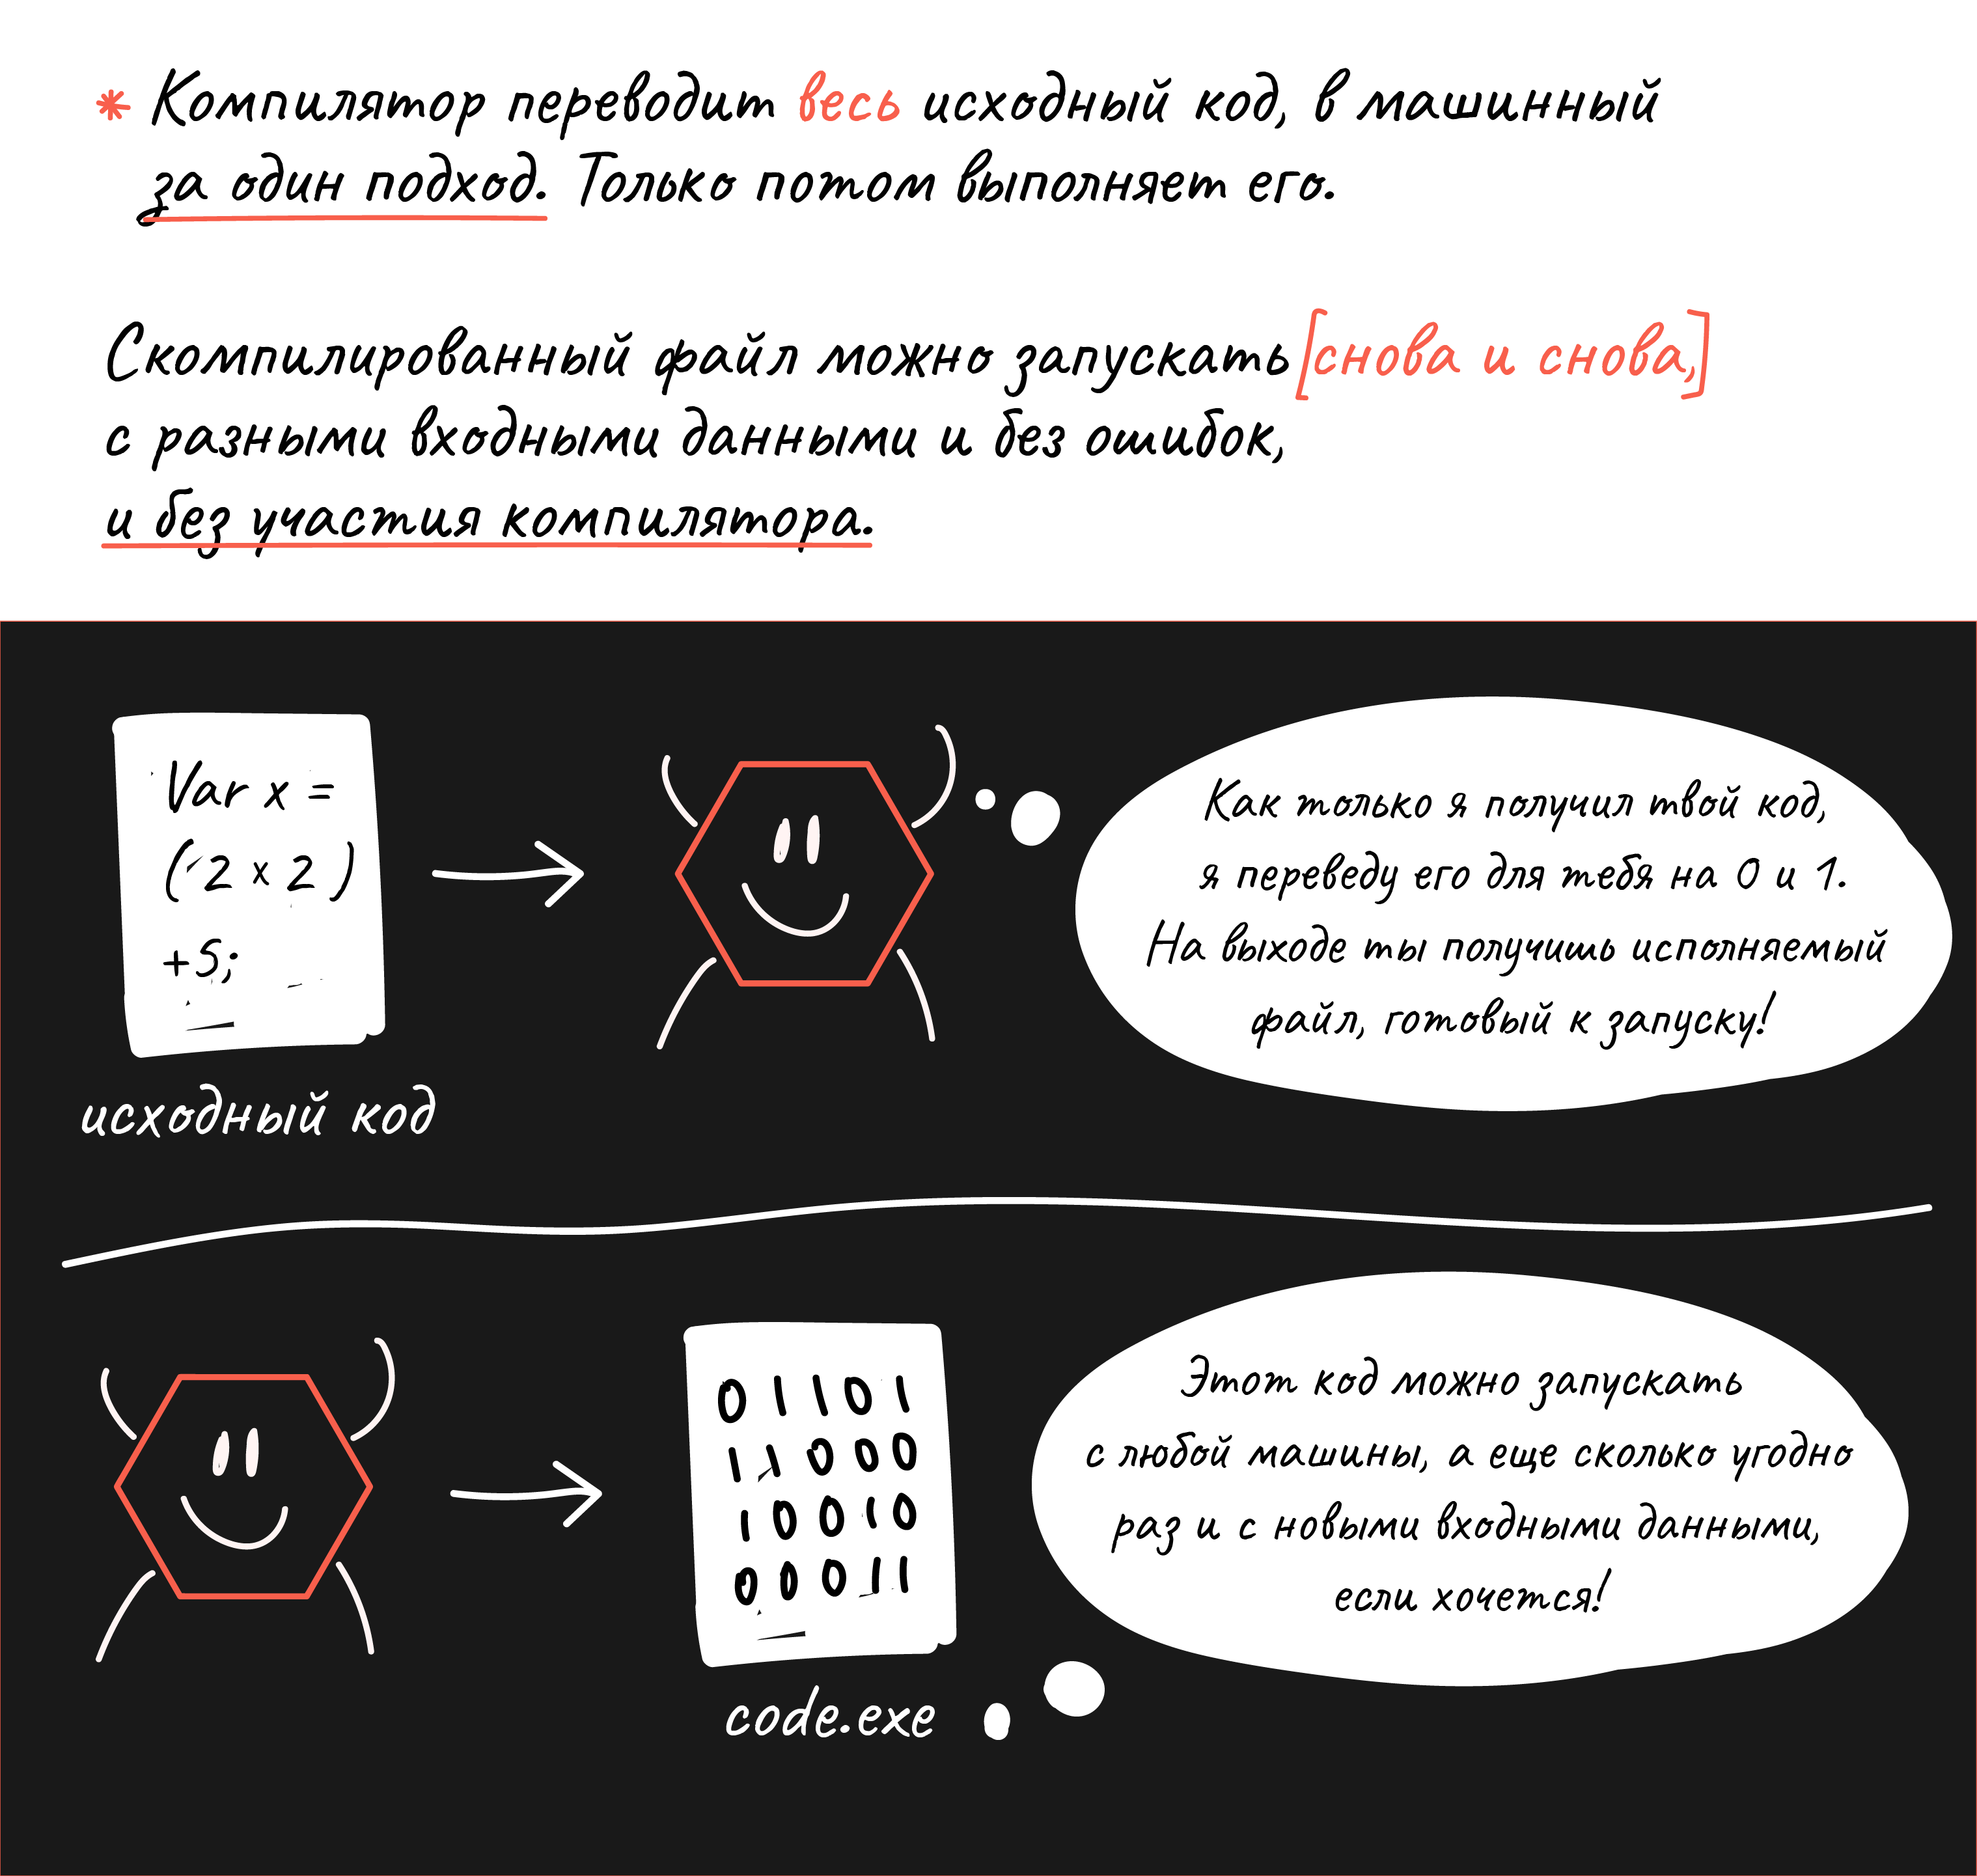
\includegraphics[width=0.9\linewidth]{images/pic1-5.png}
\end{figure}

\begin{figure}[h!]\center
  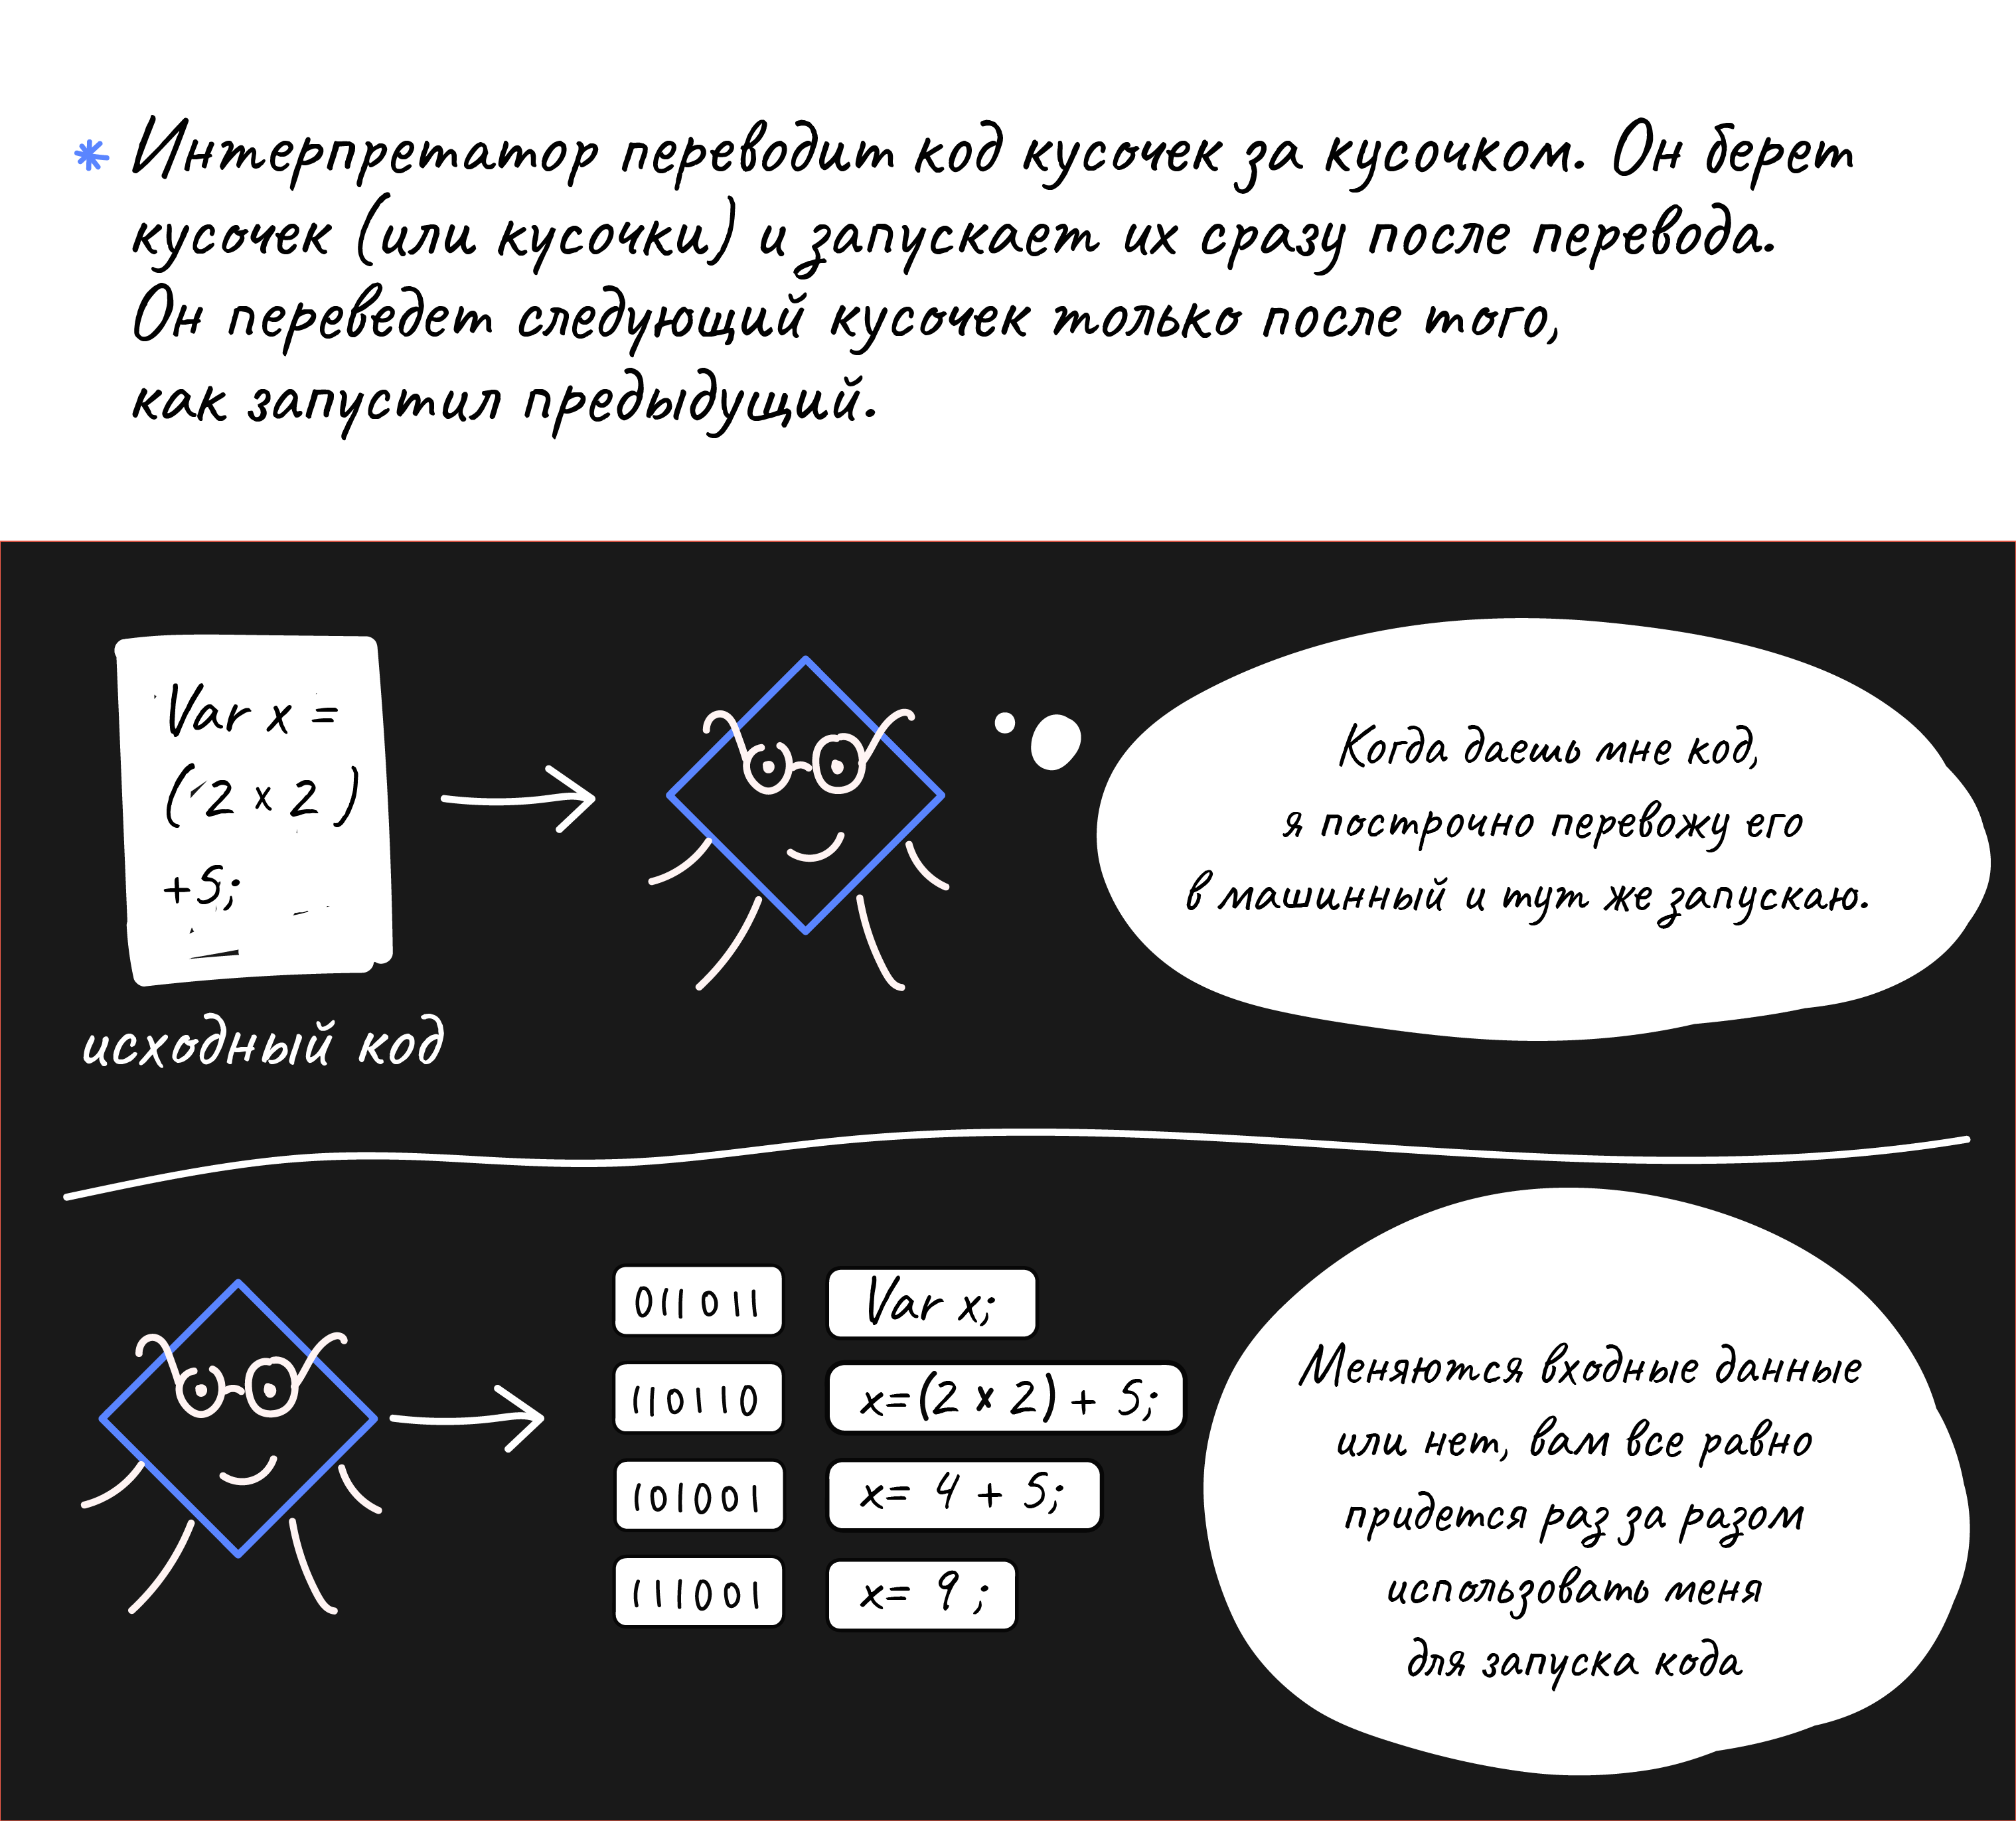
\includegraphics[width=0.9\linewidth]{images/pic1-6.png}
\end{figure}
%--------------------------------------------------------------------------------------------
\newpage
\section*{Вопросы и задания для самоконтроля}% Этот раздел будет состоять из вопросов
% и заданий для самоконтроля.
\addcontentsline{toc}{struct}{Вопросы и задания для самоконтроля}% Эта команда
% добавляет название раздела в раздел <<Содержание>>

Здесь можете привести список вопросов и заданий для самоконтроля:
\begin{enumerate}% Эта команда начинает список
\item Вопрос или задание.
\item Вопрос или задание.
\item Вопрос или задание.
\item Вопрос или задание.
\end{enumerate}% Эта команда завершает список

\newpage
\chapter{Основы программного проекта. Структура программы}
\section{Первый проект и основные соглашения при работе над проектом}

Для создания первого проекта на Java вам потребуется выполнить следующие шаги:
\begin{enumerate}
\item Установите Java Development Kit (JDK) на ваш компьютер. JDK содержит необходимые инструменты для разработки приложений на Java, включая компилятор и среду выполнения Java (JRE).
\item Установите интегрированную среду разработки (IDE), такую как Eclipse или IntelliJ IDEA. IDE позволяет упростить процесс разработки, предоставляя много полезных функций, таких как автодополнение кода, отладчик и многие другие.
\item Создайте новый проект в вашей IDE и настройте его. Укажите название проекта, место сохранения и выберите версию Java.
\item Создайте класс в вашем проекте. Это можно сделать, выбрав пункт меню "New Class" в вашей IDE. В классе вы можете создавать переменные, методы и другие элементы, необходимые для вашего приложения.
\item Напишите код для вашего приложения в методе "main" вашего класса. Метод "main" является точкой входа в ваше приложение, и он будет вызываться при запуске программы. Например, вы можете написать простейшее приложение, которое выводит сообщение на экран:
\begin{lstlisting}
public class MyFirstJavaApp {
    public static void main(String[] args) {
       System.out.println("Hello World!");
   }
}
\end{lstlisting}
\item Сохраните ваш код и запустите приложение. В вашей IDE должна быть кнопка для запуска программы. После запуска вы должны увидеть сообщение "Hello World!" в консольном окне.
\item Продолжайте улучшать ваше приложение, добавляя новый функционал, исправляя ошибки и тестировая его. Помните о соглашениях о форматировании кода, комментариях и тестировании.
\end{enumerate}

При работе над проектом на Java очень важно придерживаться определенных соглашений, чтобы ваш код был читаемым и понятным для других разработчиков. Вот некоторые из основных соглашений, которых нужно придерживаться:
\begin{enumerate}
\item Используйте соглашение CamelCase для именования переменных, методов и классов. Начинайте имя класса с заглавной буквы, а имя метода или переменной - с маленькой.
\item Используйте описательные имена переменных, методов и классов. Названия должны отражать смысл элементов, которые они описывают.
\item Используйте отступы и пробелы для лучшей читаемости кода. Ваш код должен быть отформатирован, чтобы было легко понимать его структуру.
\item Комментируйте свой код. Комментарии должны описывать, что делает ваш код и почему он делает то, что делает. Комментарии также должны быть написаны с использованием правильной грамматики и пунктуации.
\item Используйте версионный контроль. Версионный контроль позволяет отслеживать изменения в вашем коде, управлять версиями и восстанавливать предыдущие версии.
\item Пишите тесты. Написание тестов помогает обнаружить ошибки и гарантирует, что ваш код работает так, как задумано.
\item Следуйте принципам SOLID. SOLID - это набор принципов, которые помогают создавать гибкие и расширяемые приложения. Следование этим принципам поможет вам создать хороший дизайн приложения.
\item Соблюдайте стиль кодирования. Существует множество стилей кодирования на Java, таких как стиль Sun или Google. Выберите один стиль и следуйте ему во всем своем коде.
\end{enumerate}

Соблюдение этих соглашений поможет вам создавать читаемый и понятный код, который будет легко поддерживаться другими разработчиками.

\section{Использование JDK, JRE}

Использование JDK и JRE зависит от ваших потребностей и задач, которые вы выполняете. Вот несколько примеров использования JDK и JRE:
\begin{itemize}
\item Если вы планируете разрабатывать приложения на Java, вам необходимо установить JDK. JDK включает в себя необходимые инструменты для создания, отладки и компиляции приложений на Java. Он включает в себя компилятор, библиотеки и другие инструменты, необходимые для разработки приложений на Java.
\item Если вы хотите просто запустить приложение на Java, вам достаточно установить JRE. JRE содержит только необходимые компоненты для запуска приложений на Java, такие как виртуальная машина Java и библиотеки, необходимые для выполнения приложения.
\item Если вы используете среду разработки Java (IDE) для создания приложений на Java, вам, вероятно, понадобится JDK. Некоторые IDE, такие как Eclipse и NetBeans, могут включать в себя JDK, но если нет, вам нужно будет установить JDK вручную.
\item Если вы хотите запустить Java-приложение в браузере, вам понадобится JRE. Браузеры используют JRE для запуска Java-апплетов (веб-приложений на Java), которые работают внутри браузера.
\item Если вы разрабатываете приложение, которое должно быть запущено на другой машине, убедитесь, что на этой машине установлен JRE. Это позволит вашему приложению быть запущенным на этой машине, без необходимости установки JDK или других инструментов разработки.
\end{itemize}

\section{Написание простой программы}

Исходный код программы
\begin{lstlisting}
public class Welcome {
    public static void main(String[] args) {
        //Welcome to Java!
        System.out.println("Welcome to Java!");
    }
}
\end{lstlisting}

Строка 1 определяет класс. Каждая Java программа должна иметь по крайней мере один класс. Каждый класс имеет имя. Принято, что имена классов начинаются с заглавной буквы. В этом примере класс назван \textbf{Welcome}.

Строка 2 определяет метод \textbf{main}. Программа начинает выполнение с метода \textbf{main}. Метод \textbf{main} – это точка входа, где программа начинает выполнение.

Метод – это конструкция, которая содержит инструкции. Метод \textbf{main} в этой программе содержит инструкцию \textbf{System.out.println}. Инструкция отображает в консоли строку \textbf{«Welcome to Java!»}. Строка (String) – это термин в программировании, означающий последовательность символов. Строка должна быть заключена в двойные кавычки. Каждая инструкция в Java заканчивается точкой с запятой ( ; ), которая служит разделителем инструкций.

Зарезервированные слова, или как их ещё называют ключевые слова, имеют определённое значение для компилятора, и они не могут использоваться для других целей в программе. Например, когда компилятор видит слово \textbf{class}, он понимает, что слово после \textbf{class} – это имя класса. Другими зарезервированными словами в этой программе являются \textbf{public}, \textbf{static} и \textbf{void}.

Строка 3 – это комментарий, которая документирует действия программы и её устройство. Комментарии помогают программистам общаться и понимать программу. Они не являются программными инструкциями и, таким образом, игнорируются компилятором. В Java комментариям предшествуют два слеша на строке (\textbf{//}), которая так и называется – строка комментария. Комментарии могут располагаться между \textbf{/*} и \textbf{*/} на одной или нескольких строках, эти строки называются блоком комментариев или параграфом комментариев. Когда компилятор видит \textbf{//}, то он на этой строке игнорирует весь текст после \textbf{//}. Когда видит \textbf{/*}, он сканирует следующий \textbf{*/} и игнорирует любой текст между \textbf{/*} и \textbf{*/}.

Пара фигурных скобок в программе формирует блок, который группирует компоненты программы. В Java каждый блок начинается с открывающей фигурной скобки и заканчивается закрывающей фигурной скобкой. Каждый класс имеет блок класса, который группирует данные и методы класса. Похожим образом каждый метод имеет блок метода, который группирует инструкции в методе. Блоки могут быть вложенными, это означает, что один блок может быть помещён внутри другого, как показано на следующем коде:
\begin{figure}[h!]\center
  \includegraphics[width=0.8\linewidth]{images/pic1-7.jpg}
\end{figure}

\section{Аргументы командной строки}

Аргументы командной строки - это значения, передаваемые программе при ее запуске из командной строки. В Java аргументы командной строки передаются в виде массива строк (типа String[]), который можно получить из метода main().

Синтаксис передачи аргументов командной строки в Java выглядит следующим образом:

\begin{lstlisting}
java MyProgram arg1 arg2 arg3 ...
\end{lstlisting}

где MyProgram - имя главного класса вашей программы, а arg1, arg2, arg3 - аргументы командной строки.

В вашей программе вы можете получить массив аргументов командной строки следующим образом:

\begin{lstlisting}
public static void main(String[] args) {
    // args[0] contains the first command line argument
    // args[1] contains the second command line argument
    // etc.
}
\end{lstlisting}

Важно помнить, что все аргументы командной строки передаются в виде строковых значений, поэтому вам нужно преобразовывать их в нужный тип данных, если это необходимо.

Например, если вы хотите передать программе имя пользователя и его возраст, вы можете написать следующий код:

\begin{lstlisting}
public static void main(String[] args) {
    String name = args[0];
    int age = Integer.parseInt(args[1]);
    
    System.out.println("Hello, " + name + "!");
    System.out.println("You are " + age + "years old.");
}
\end{lstlisting}

В этом примере мы получаем первый аргумент командной строки - имя пользователя - и сохраняем его в переменной name. Затем мы получаем второй аргумент командной строки - возраст - и преобразуем его в целочисленное значение, используя метод Integer.parseInt(). Далее мы выводим на экран приветствие и возраст пользователя.

Если вы передадите программе неверное количество аргументов командной строки, то программа выдаст ошибку. Чтобы избежать ошибок, вы можете проверять количество аргументов, используя свойство args.length. Например:

\begin{lstlisting}
public static void main(String[] args) {
    if (args.length != 2) {
        System.out.println("Usage: MyProgram <name> <age>");
        System.exit(1);
    }
    
    // Handling Command Line Arguments
}
\end{lstlisting}

В этом примере мы проверяем количество аргументов командной строки и выводим сообщение об ошибке, если передано неверное количество аргументов. Затем мы можем продолжить обработку аргументов, если проверка прошла успешно.

\section{Группировка классов}

В Java существует концепция пакетов (packages), которые позволяют группировать классы в логически связанные группы. Пакеты используются для организации и управления большими проектами, которые содержат множество классов.

Пакеты в Java являются иерархическими и их имена формируются по структуре директорий в файловой системе. Имя пакета указывается в начале каждого файла с исходным кодом Java, используя ключевое слово package. Например, если вы хотите создать пакет с именем com.example.myapp, то в начале каждого файла с исходным кодом Java нужно добавить строку:

\begin{lstlisting}
package com.example.myapp;
\end{lstlisting}

После этого классы, которые определены в этом файле, будут принадлежать к пакету com.example.myapp.

Чтобы использовать классы из другого пакета, нужно либо указать полное имя класса (с указанием имени пакета), либо импортировать класс с помощью ключевого слова import. Например, если вы хотите использовать класс MyClass из пакета com.example.myapp, то можно написать:

\begin{lstlisting}
com.example.myapp.MyClass obj = new com.example.myapp.MyClass();
\end{lstlisting}

Или импортировать класс и использовать его без указания имени пакета:

\begin{lstlisting}
import com.example.myapp.MyClass;

...

MyClass obj = new MyClass();
\end{lstlisting}

Группировка классов в пакеты позволяет легче ориентироваться в большом количестве классов и более эффективно организовывать код. Пакеты также предоставляют механизмы для контроля доступа к классам и их членам.

\section{Пакеты, и их импорт}

Как правило, в Java классы объединяются в пакеты. Пакеты позволяют организовать классы логически в наборы. По умолчанию java уже имеет ряд встроенных пакетов, например, java.lang, java.util, java.io и т.д. Кроме того, пакеты могут иметь вложенные пакеты.

Организация классов в виде пакетов позволяет избежать конфликта имен между классами. Ведь нередки ситуации, когда разработчики называют свои классы одинаковыми именами. Принадлежность к пакету позволяет гарантировать однозначность имен.

\begin{lstlisting}
package com.example.myapp;
\end{lstlisting}

Как правило, названия пакетов соответствуют физической структуре проекта, то есть организации каталогов, в которых находятся файлы с исходным кодом. А путь к файлам внутри проекта соответствует названию пакета этих файлов. Например, если классы принадлежат пакету com.example.myapp, то эти классы помещаются в проекте в папку com.example.myapp.

Классы необязательно определять в пакеты. Если для класса пакет не определен, то считается, что данный класс находится в пакете по умолчанию, который не имеет имени.

Чтобы использовать классы пакетов в своей программе, нужно импортировать их в код. Для импорта пакета используется ключевое слово import вместе с именем пакета. Например, чтобы импортировать класс String из пакета java.lang, нужно добавить следующую строку в начало кода:

\begin{lstlisting}
import java.lang.String;
\end{lstlisting}

После импорта класса его можно использовать в программе без указания полного имени пакета, например:

\begin{lstlisting}
String s = "Hello, world!";
System.out.println(s);
\end{lstlisting}

Важно заметить, что не все классы из стандартной библиотеки Java автоматически импортируются в программу. Некоторые из них, такие как System, Math и String, находятся в пакете java.lang и могут использоваться без явного импорта. Однако большинство других классов и пакетов нужно импортировать явно.

Также можно использовать символ звездочки (*) для импорта всех классов из пакета:

\begin{lstlisting}
import java.util.*;
\end{lstlisting}

Это позволяет использовать все классы из пакета без указания их имен, но следует быть осторожным с этим подходом, так как он может привести к конфликту имен или неэффективному использованию ресурсов.

\newpage
\chapter{Синтаксис Java. Управляющие конструкции. Массивы}
\section{Синтаксические конструкции Java}

Java является объектно-ориентированным языком программирования, который использует много различных синтаксических конструкций. Вот несколько основных:

\begin{itemize}
\item Переменные и типы данных: Java имеет множество типов данных, включая примитивные типы, такие как int, double, boolean, а также классы и интерфейсы. Переменные объявляются с использованием ключевого слова "var" или указания типа и имени переменной.

\begin{lstlisting}
int x;
String message;
double d = 3.14;
\end{lstlisting}

\item Условные операторы: Java поддерживает различные условные операторы, такие как "if", "else if" и "switch". Они используются для принятия решения на основе значения переменных.

\begin{lstlisting}
if (condition) {
    // code to be executed if the condition is true
} else {
    // code to be executed if condition is false
}
\end{lstlisting}

\begin{lstlisting}
switch (variable) {
    case value1:
        // code to be executed if variable == value1
        break;
    case value2:
        // code to be executed if variable == value2
        break;
    default:
        // code to be executed if variable does not match any of the values
        break;
}
\end{lstlisting}

\item Циклы: Java поддерживает различные циклы, такие как "for", "while" и "do-while". Они используются для повторения блока кода несколько раз.

\begin{lstlisting}
for (int i = 0; i < 10; i++) {
    // code to be executed 10 times
}

while (condition) {
    // code to be executed while the condition is true
}

do {
    // code to be executed while the condition is true
} while (condition);
\end{lstlisting}

\item Массивы: Массивы в Java используются для хранения нескольких элементов одного типа в одной переменной. Они объявляются с использованием квадратных скобок [].
\item Методы: Методы - это блоки кода, которые могут быть вызваны из других частей программы. Они объявляются с помощью ключевого слова "void" или типа возвращаемого значения, имени метода и параметров.
\item Обработка исключений: Java поддерживает обработку исключений для обработки ошибок в программе. Исключения могут быть обработаны с помощью блока "try-catch".

\begin{lstlisting}
try {
    // code that can throw an exception
} catch (Exception e) {
    // code to be executed if an exception occurs
} finally {
    //code that will be executed regardless of whether an exception occurred or not
}
\end{lstlisting}

\item Классы и объекты: Java является объектно-ориентированным языком программирования, и классы и объекты используются для организации кода и создания экземпляров программы.

\begin{lstlisting}
public class MyClass {
    // class fields and methods
}
\end{lstlisting}
\end{itemize}

\section{Ветвления и циклы}

\textbf{Условные операторы (ветвления)}

\textbf{if}

Оператор if позволяет проверить, выполняется ли некоторое условие, и выполнить блок кода, если оно истинно. Если условие ложно, блок кода пропускается. Синтаксис оператора if выглядит следующим образом:

\begin{lstlisting}
if (condition) {
    // block of code that will be executed if the condition is true
}
\end{lstlisting}

\textbf{if-else}

Оператор if-else позволяет выполнить один блок кода, если условие истинно, и другой блок кода, если условие ложно. Синтаксис оператора if-else выглядит следующим образом:

\begin{lstlisting}
if (condition) {
    // block of code that will be executed if the condition is true
} else {
    // block of code that will be executed if the condition is false
}
\end{lstlisting}

\textbf{if-else if}

Оператор if-else if позволяет проверить несколько условий и выполнить соответствующий блок кода, если хотя бы одно из них истинно. Если все условия ложны, выполнится блок кода, связанный с оператором else. Синтаксис оператора if-else if выглядит следующим образом:

\begin{lstlisting}
if (condition1) {
    // block of code to be executed if condition1 is true
} else if (condition2) {
    // block of code to be executed if condition1 is false and condition2 is true
} else {
    // block of code to be executed if all conditions are false
}
\end{lstlisting}

\textbf{Циклы}

\textbf{for}

Оператор for позволяет выполнить блок кода несколько раз, пока выполняется определенное условие. Синтаксис оператора for выглядит следующим образом:

\begin{lstlisting}
for (initialization; condition; change) {
  // block of code to be executed
}
\end{lstlisting}

\textbf{while}

Цикл while позволяет выполнять блок кода, пока указанное условие истинно:

\begin{lstlisting}
while (condition) {
  // block of code to be executed
}
\end{lstlisting}

\textbf{do-while}

Цикл do-while похож на цикл while, но сначала выполняет блок кода, а затем проверяет условие:

\begin{lstlisting}
do {
  // block of code to be executed
} while (condition);
\end{lstlisting}

\textbf{for-each}

Цикл for-each используется для перебора элементов массива или коллекции:

\begin{lstlisting}
for (element_type element_name : array_or_collection_name) {
  // block of code to be executed
}
\end{lstlisting}

\section{Формы цикла for}

В языке программирования Java существуют три формы цикла for:

\begin{enumerate}
    \item Основная форма for: for (инициализация; условие; обновление) { тело цикла }

Пример:

\begin{lstlisting}
for (int i = 0; i < 10; i++) {
    System.out.println(i);
}
\end{lstlisting}

Эта форма цикла предназначена для выполнения заданного количества итераций. Она состоит из трех частей: инициализации, условия и обновления. Инициализация выполняется перед началом выполнения цикла и используется для объявления и инициализации переменных, которые будут использоваться в цикле. Условие проверяется перед каждой итерацией, и если оно истинно, то тело цикла выполняется. Обновление выполняется после каждой итерации и обычно используется для изменения значения переменных, используемых в условии.
    \item Форма цикла for-each (цикл по элементам коллекции): for (тип переменной : коллекция) { тело цикла }

Пример:

\begin{lstlisting}
int[] numbers = {1, 2, 3, 4, 5};
for (int num : numbers) {
    System.out.println(num);
}
\end{lstlisting}

Эта форма цикла позволяет перебрать все элементы коллекции или массива. Переменная num принимает значения каждого элемента коллекции или массива по очереди.
    \item Бесконечный цикл с прерыванием: for (;;) { тело цикла }

Пример:

\begin{lstlisting}
int i = 0;
for (;;) {
    if (i == 10) {
        break;
    }
    System.out.println(i);
    i++;
}
\end{lstlisting}

Эта форма цикла используется для выполнения бесконечного цикла с прерыванием при выполнении определенного условия. В данном примере цикл будет выполняться до тех пор, пока переменная i не достигнет значения 10. Ключевое слово break используется для выхода из цикла.
\end{enumerate}

\section{Объявление и инициализация массивов}

Массив в Java - это упорядоченный список элементов одного типа, который хранится в непрерывной области памяти. Массивы имеют фиксированный размер, определяемый в момент их создания.

Для объявления массива необходимо указать тип данных элементов массива, за которым следует квадратная скобка []. Если массив содержит элементы определенного типа, то тип этого массива будет указан до скобок [].

Существует два способа инициализации массивов в Java:

\begin{enumerate}
    \item Использование оператора new, который создает новый массив с заданным размером:

\begin{lstlisting}
int[] myArray = new int[5];
\end{lstlisting}

В данном примере создается массив myArray, содержащий 5 элементов типа int, которые по умолчанию равны 0.
    \item Использование литералов массивов:

\begin{lstlisting}
int[] myArray = {1, 2, 3, 4, 5};
\end{lstlisting}

В данном примере создается массив myArray, содержащий 5 элементов типа int, со значениями 1, 2, 3, 4, 5.

Массивы в Java могут содержать элементы любого примитивного типа или объектного типа, включая другие массивы. Для доступа к элементам массива используется индексация, начинающаяся с нуля.

Примеры доступа к элементам массива:

\begin{lstlisting}
int[] myArray = {1, 2, 3, 4, 5};
int firstElement = myArray[0]; // first array element equal to 1
int lastElement = myArray[myArray.length - 1]; // the last element of the array is 5
\end{lstlisting}

Также можно изменять значения элементов массива:

\begin{lstlisting}
myArray[1] = 10; // changing the second element to 10
\end{lstlisting}
\end{enumerate}

\newpage
\chapter{Примитивные типы. Операции над переменными примитивного типа}
\section{Понятие типа данных}

Тип данных - это специальный атрибут, который определяет тип значения, которое может храниться в переменной, методе или возвращаемом значении метода в Java.

Java имеет две категории типов данных:
\begin{enumerate}
    \item Примитивные типы данных: boolean, byte, short, int, long, float, double, char.
    \item Ссылочные типы данных: классы, интерфейсы, массивы.
\end{enumerate}

Примитивные типы данных в Java представляют основные типы, которые используются для хранения простых значений, таких как числа, символы и значения true/false.

Ссылочные типы данных в Java представляют более сложные типы, которые состоят из примитивных типов и/или других ссылочных типов данных. Классы и интерфейсы являются двумя основными типами ссылочных типов данных в Java. Классы могут содержать методы, поля и конструкторы, которые позволяют создавать объекты этого класса. Интерфейсы определяют методы, которые должны быть реализованы классами, которые реализуют эти интерфейсы.

Массивы в Java представляют собой ссылочный тип данных, который может хранить набор значений одного типа данных. Массивы могут быть одномерными, двумерными и многомерными и имеют специальный синтаксис для объявления и инициализации.

Правильный выбор типа данных в Java является важной задачей, поскольку он может повлиять на производительность, использование памяти и удобство работы с данными в коде.

\section{Примитивные (элементарные) типы и их использование}

В языке Java есть 8 примитивных типов данных:

\begin{enumerate}
    \item byte - 8-битное целое число со знаком, может принимать значения от -128 до 127. Используется для экономии памяти при работе с большими массивами чисел.
    \item short - 16-битное целое число со знаком, может принимать значения от -32 768 до 32 767.
    \item int - 32-битное целое число со знаком, может принимать значения от -2 147 483 648 до 2 147 483 647.
    \item long - 64-битное целое число со знаком, может принимать значения от -9 223 372 036 854 775 808 до 9 223 372 036 854 775 807.
    \item float - 32-битное число с плавающей запятой, используется для представления дробных чисел с плавающей запятой. Может принимать значения от 1.4e-45 до 3.4e+38.
    \item double - 64-битное число с плавающей запятой, используется для представления более точных дробных чисел с плавающей запятой. Может принимать значения от 4.9e-324 до 1.8e+308.
    \item char - 16-битный символ Unicode, может содержать любой символ из множества Unicode. Используется для представления символов и строк.
    \item boolean - логический тип данных, может принимать только два значения: true (истина) и false (ложь). Используется для условных операций.
\end{enumerate}

Примитивные типы данных могут использоваться для объявления переменных и констант, для аргументов методов, а также в выражениях и операциях. Они имеют определенный размер в памяти и обеспечивают быстродействие при выполнении программы. Однако, они не имеют методов и свойств, как объекты классов, и не могут быть использованы в качестве аргументов для многих методов стандартной библиотеки Java.

\section{Основные категории примитивных типов}

В Java примитивные типы данных делятся на 4 категории:

\begin{enumerate}
    \itemЦелочисленные типы (byte, short, int, long) - используются для хранения целочисленных значений.
    \item Тип float и тип double - используются для хранения чисел с плавающей точкой.
    \item Тип char - используется для хранения символов Юникода.
    \item Тип boolean - используется для хранения булевых значений (true/false).
\end{enumerate}

Каждый из примитивных типов имеет свой диапазон значений и занимает разное количество памяти. Также для каждого типа определены операции, которые можно выполнять с его значениями (например, арифметические операции для целочисленных типов и операции сравнения для всех типов).

\section{Операции над примитивными типами}

Операции над примитивными типами в Java могут быть разделены на следующие категории:

\begin{enumerate}
    \item Арифметические операции:
    \begin{itemize}
        \item Сложение: +
        \item Вычитание: -
        \item Умножение: *
        \item Деление: /
        \item Остаток от деления
    \end{itemize}
    Примеры:
    \begin{lstlisting}
int a = 10;
int b = 5;
int c = a + b; // c = 15
int d = a - b; // d = 5
int e = a * b; // e = 50
int f = a / b; // f = 2
int g = a % b; // g = 0
    \end{lstlisting}
    \item Операции сравнения:
    \begin{itemize}
        \item Равенство: ==
        \item Неравенство: !=
        \item Больше: >
        \item Меньше: <
        \item Больше или равно: >=
        \item Меньше или равно: <=
    \end{itemize}
    
    Операции сравнения возвращают логический тип boolean. Значение true означает, что условие истинно, а значение false - что оно ложно.

Примеры:
 \begin{lstlisting}
int a = 10;
int b = 5;
boolean c = a == b; // c = false
boolean d = a != b; // d = true
boolean e = a > b; // e = true
boolean f = a < b; // f = false
boolean g = a >= b; // g = true
boolean h = a <= b; // h = false
    \end{lstlisting}
    \item Логические операции:
    \begin{itemize}
        \item Логическое И
        \item Логическое ИЛИ: ||
        \item Логическое НЕ: !
    \end{itemize}
    Логические операции также возвращают логический тип boolean. Операции И и ИЛИ могут быть использованы для объединения условий, а операция ! используется для инвертирования значения логического выражения.

Примеры:

 \begin{lstlisting}
boolean a = true;
boolean b = false;
boolean c = a && b; // c = false
boolean d = a || b; // d = true
boolean e = !a; // e = false
boolean f = !(a && b); // f = true
    \end{lstlisting}
    \item Побитовые операции:
    \begin{itemize}
        \item Побитовое И
        \begin{lstlisting}
int a = 3;  // 0000 0011 in binary
int b = 6;  // 0000 0110 in binary
int c = a & b;  // 0000 0010 in binary (the result of a bitwise AND)
System.out.println(c);  // outputs 2
    \end{lstlisting}
        \item Побитовое ИЛИ: |
        \begin{lstlisting}
int a = 3;  // 0000 0011 in binary
int b = 6;  // 0000 0110 in binary
int c = a | b;  // 0000 0111 in binary (bitwise OR result)
System.out.println(c);  // outputs 7
    \end{lstlisting}
        \item Исключающее ИЛИ
        \begin{lstlisting}
int a = 3;  // 0000 0011 in binary
int b = 6;  // 0000 0110 in binary
int c = a ^ b;  // 0000 0101 in binary system (XOR result)
System.out.println(c);  // outputs 5
    \end{lstlisting}
        \item Побитовый сдвиг влево: <<
        \begin{lstlisting}
int a = 3;  // 0000 0011 in binary
int b = a << 2;  // 0000 1100 in binary (the result of a bit shift left by 2 bits)
System.out.println(b);  // outputs 12
    \end{lstlisting}
        \item Побитовый сдвиг вправо: >>
        \begin{lstlisting}
int a = 12;  // 0000 1100 in binary
int b = a >> 2;  // 0000 0011 in binary (the result of a bitwise shift to the right by 2 bits)
System.out.println(b);  // outputs 3
    \end{lstlisting}
        \item Побитовый сдвиг вправо с заполнением нулями: >>>
        \begin{lstlisting}
int a = -12;  // 1111 0100 in binary
int b = a >>> 2;  // 0011 1101 in binary (the result of a bitwise shift to the right by 2 bits)
System.out.println(b);  // output 61
    \end{lstlisting}
        \item Побитовое НЕ: ~
        \begin{lstlisting}
int a = 3;  // 0000 0011 in binary
int b = ~a;  // 1111 1100 in binary (result of bitwise NOT)
System.out.println(b);  // prints -4
    \end{lstlisting}
    \end{itemize}
\end{enumerate}

\section{Явное и неявное приведение типов}

В Java есть два типа приведения типов - явное (explicit) и неявное (implicit). Явное приведение - это приведение типа, которое выполняется в явном виде в программном коде, с помощью оператора приведения. Неявное приведение - это приведение типа, которое выполняется автоматически компилятором, когда значения одного типа присваиваются переменной другого типа, или когда выражения разных типов объединяются в одном выражении.

Явное приведение выполняется следующим образом:

\begin{lstlisting}
double d = 10.5;
int i = (int) d;  // explicit cast double to int
\end{lstlisting}

В этом примере мы объявляем переменную double и присваиваем ей значение 10.5. Затем мы приводим значение переменной double к типу int с помощью оператора приведения, и присваиваем результат переменной int. В результате, значение переменной i будет равно 10, т.к. дробная часть 0.5 будет отброшена.

Неявное приведение выполняется автоматически компилятором, если типы данных совместимы. Например:

\begin{lstlisting}
int i = 10;
double d = i;  // implicit casting of int to double
\end{lstlisting}

В этом примере мы объявляем переменную int и присваиваем ей значение 10. Затем мы объявляем переменную double и присваиваем ей значение переменной int. Компилятор автоматически выполняет приведение типа int к типу double, и присваивает результат переменной double. В результате, значение переменной d будет равно 10.0.

Неявное приведение также происходит при использовании операторов. Например:

\begin{lstlisting}
int i = 10;
double d = 2.5;
double result = i * d;  // implicit casting of int to double
\end{lstlisting}

В этом примере мы объявляем переменные int и double, и присваиваем им значения. Затем мы объединяем переменные в выражении, используя оператор умножения. Компилятор автоматически выполняет приведение типа int к типу double, и выполняет операцию умножения, и присваивает результат переменной result. В результате, значение переменной result будет равно 25.0.

Неявное приведение может привести к потере точности или искажению данных, поэтому в некоторых случаях необходимо использовать явное приведение.
%---------------------------------------------------------------------------------------------
\newpage% Эта команда задает разрыв страницы (начинает новую страницу).
\section*{ПРАКТИЧЕСКОЕ ЗАНЯТИЕ 1}% Эта команда начинает первое практическое занятие.
% Обратите внимание -- практические занятия придется нумеровать вручную.
\addcontentsline{toc}{chapter}{Практическое занятие 1 {\bf Тема занятия}} \vspace{-10pt}% Эти
% команды добавляют тему занятия в раздел <<Содержание>>
\begin{center}% Эта команда выравнивает текст по центру строки.
 {\bf% Эта команда делает шрифт полужирным
 Тема занятия}
\end{center}% Эта команда завершает <<центрирование>> текста.

{\bf Цель:} Сюда можно вписать цель практического занятия.
\\% Эта команда вставляет пустую строку.

Ваш текст.

%--------------------------------------------------------------------------------------------
\newpage% Эта команда начинает новую страницу
\section*{Задания для самостоятельного решения (выполнения)}% Эта команда начинает раздел с
% заданиями для самостоятельной работы
\addcontentsline{toc}{struct}{Задания для самостоятельного решения}% Эта команда добавляет
% название раздела в раздел <<Содержание>>

Ваш текст

\newpage% Эта команда задает новую страницу (разрыв страницы)

%--------------------------------------------------------------------------------------------


\section*{Вопросы и задания для самоконтроля}% Этот раздел будет состоять из вопросов
% и заданий для самоконтроля.
\addcontentsline{toc}{struct}{Вопросы и задания для самоконтроля}% Эта команда
% добавляет название раздела в раздел <<Содержание>>

Здесь можете привести список вопросов и заданий для самоконтроля:
\begin{enumerate}% Эта команда начинает список
\item Вопрос или задание.
\item Вопрос или задание.
\item Вопрос или задание.
\item Вопрос или задание.
\end{enumerate}% Эта команда завершает список

А можете подготовить с помощью программы IrenEditor (см. <<Руководство пользователю>>)
тестовое задание для самоконтроля, сохранить его в папку
<<test>>, назвав, например, lk1.exe, и создать на него метку с помощью
команды (см. <<Руководство пользователю>>): \href{run:test/lk1.exe}{Пройдем тестирование?}

%---------------------------------------------------------------------------------------------
\newpage% Эта команда задает разрыв страницы (начинает новую страницу).
\section*{ПРАКТИЧЕСКОЕ ЗАНЯТИЕ 2}% Эта команда начинает второе практическое занятие.
% Обратите внимание -- практические занятия придется нумеровать вручную.
\addcontentsline{toc}{chapter}{Практическое занятие 2 {\bf Тема занятия}} \vspace{-10pt}% Эти
% команды добавляют тему занятия в раздел <<Содержание>>
\begin{center}% Эта команда выравнивает текст по центру строки.
 {\bf% Эта команда делает шрифт полужирным
 Тема занятия}
\end{center}% Эта команда завершает <<центрирование>> текста.

{\bf Цель:} Сюда можно вписать цель практического занятия.
\\% Эта команда вставляет пустую строку.

Ваш текст.

%--------------------------------------------------------------------------------------------
\newpage% Эта команда начинает новую страницу
\section*{Задания для самостоятельного решения (выполнения)}% Эта команда начинает раздел с
% заданиями для самостоятельной работы
\addcontentsline{toc}{struct}{Задания для самостоятельного решения}% Эта команда добавляет
% название раздела в раздел <<Содержание>>

Ваш текст

%--------------------------------------------------------------------------------------------

\newpage% Эта команда задает новую страницу (разрыв страницы)


\normalsize\section*{Варианты заданий для индивидуальной работы}% Эта команда создает новый
% раздел, название которого записано в фигурных скобках.
\addcontentsline{toc}{struct}{Варианты заданий для индивидуальной работы} % Эта
% команда добавляет название данного раздела к разделу <<Содержание>>

\begin{center}
   \bf{Вариант 1}
\end{center}

Ваш текст.

\begin{center}
   \bf{Вариант 2}
\end{center}

Ваш текст.

\begin{center}
   \bf{Вариант 3}
\end{center}

Ваш текст.

%--------------------------------------------------------------------------------------------

\newpage% Эта команда задает новую страницу (разрыв страницы)
{\large \section*{Вопросы для подготовки к экзамену и (или) зачету}% Эта команда начинает
% новый раздел, название которого записано в фигурных скобках
\addcontentsline{toc}{struct}{Вопросы для подготовки к экзамену и (или) зачету}% Эта
% команда добавляет название данного раздела к разделу <<Содержание>>

\begin{enumerate}% Эта команда начинает нумерованный список вопросов
 \item Вопрос.
\item Вопрос.
\item Вопрос.
\item Вопрос.
\end{enumerate}% Эта команда завершает нумерованный список вопросов

%--------------------------------------------------------------------------------------------

